  \documentclass[12pt]{exam}
\usepackage{amsthm}
\usepackage{libertine}
\usepackage[utf8]{inputenc}
\usepackage[margin=1in]{geometry}
\usepackage{amsmath,amssymb}
\usepackage{multicol}
\usepackage[shortlabels]{enumitem}
\usepackage{siunitx}
\usepackage{cancel}
\usepackage{float}
\usepackage{graphicx}
\usepackage{pgfplots}
\usepackage{listings}
\usepackage{tikz}


\pgfplotsset{width=10cm,compat=1.9}
\usepgfplotslibrary{external}
\tikzexternalize

\newcommand{\class}{Física Mecanica} % This is the name of the course 
\newcommand{\examnum}{Tarea 2} % This is the name of the assignment
\newcommand{\examdate}{\today} % This is the due date
\newcommand{\timelimit}{}





\begin{document}
\pagestyle{plain}
\thispagestyle{empty}

\noindent
\begin{tabular*}{\textwidth}{l @{\extracolsep{\fill}} r @{\extracolsep{6pt}} l}
	\textbf{\class} & \textbf{Name:} & \textit{Sergio Montoya}\\ %Your name here instead, obviously 
	\textbf{\examnum} &&\\
	\textbf{\examdate} &&
\end{tabular*}\\
\rule[2ex]{\textwidth}{2pt}
% ---

\begin{enumerate}
  \item[\textbf{9.1}]

    En este caso utilizaremos el \textit{Hint} que se dio en el ejercicio y nos daremos cuenta que la fuerza de empuje de arquimedes tiene una dirección opuesta a la gravedad. Por lo tanto, haremos como en el ejercicio del pendulo y plantearemos un termino \[
    g_{eff}= f-A
    .\] donde $A$ es la aceleración del carro hacia adelante. Y plantearemos el ejercicio como si esta fuera la gravedad que entonces nos quedaria
    \begin{align*}
      m\ddot{r}&=-\rho_{A} g_{eff}V - T + mg_{eff}\\
	       &= g_{eff}\left( -\rho_{A}V + m \right) - T
    .\end{align*} Que en este caso sabemos que la densidad del aire por el volumen es mayor que la masa (lo sabemos por que un globo de helio flota) y en consecuencia el angulo en el que se equilibra el globo es el inverso al que lo haria en un pendulo y en consecuencia sigue siendo: \[
    \phi_{eq}= \arctan\left( \frac{A}{g} \right) + \pi
    .\] se le suma pi para que quede en la posicion que queremos y por la simetria que tienen los angulos.
  \item[\textbf{9.2}]
    
    \begin{enumerate}
      \item Asumiendo que la estación espacial no tiene fricción y por lo tanto la misma no debe ingresar ninguna fuerza para mantener su propia rotación el sistema de fuerzas se veria:
	\begin{figure}[H]
	  \centering
	  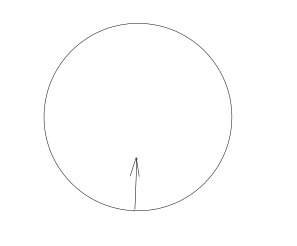
\includegraphics[width=0.4\textwidth]{Graficas/9-2a-1.jpeg}
	  \caption{Grafica de la fuerza experimentada por el astronauta en un marco de referencia inercial fuera de la estación espacial.} 
	  \label{fig:Graficas-9-2a-1}
	\end{figure}

	Donde  la flecha muestra la fuerza normal que hace la estación espacial sobre el astronauta y que apunta al centro del toroide.

      \item Ahora en el caso del marco de referencia del astronauta nos queda
	\begin{figure}[H]
	  \centering
	  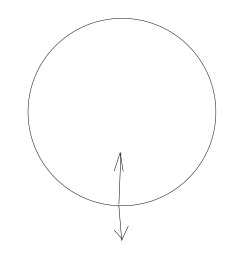
\includegraphics[width=0.4\textwidth]{Graficas/9-2b-1.jpeg}
	  \caption{Grafica de las fuerzas experimentadas por el astronauta en el marco de referencia del astronauta}
	  \label{fig:Graficas-9-2b-1-jpeg}
	\end{figure}

	Donde la flecha nueva muestra la nueva fuerza centrifuga que experimenta el astronauta. Es importante aclarar que no se pone la fuerza de Coriolis dado que el astronauta se mueve relativamente lento en esta situación por lo que no tendria efecto.

	En este caso aprovecharemos que $A=\omega^2R$ por lo tanto la fuerza centripeta experimentada seria $F_{c}=mA=m\omega^2R$. por lo tanto podemos igualarlo:
	\begin{align*}
	  F_{c}=mA=m\omega^2R=mg\\
	  \omega=\sqrt{\frac{g}{R}} \\
	  \omega = \sqrt{\frac{1}{4}}
	  \omega = \frac{1}{2}
	.\end{align*}
	
      \item Esta entonces es la velocidad angular a la que se mueve la estación espacial y en consecuencia la fuerza que experimentaria seria \[
      F_c = mA = m\omega R	
      .\] con esto entonces nos queda:
      \begin{align*}
        F_{40}=m\omega \left( 40 \right) \\
	F_{38}=m\omega \left( 38 \right) \\
	rel = \frac{m\omega \left( 38 \right) }{m\omega \left( 40 \right) } = 0.95
      .\end{align*}
    \end{enumerate}
  \item[\textbf{9.8}]
    
    \begin{enumerate}
      \item \textit{Notas Previas}

	La fuerza centrifuga se experimenta en cualquier punto hacia la misma dirección perpendicular a la velocidad tangencial. Por otro lado, la fuerza de coriollis si depende de la dirección y en particular sigue la regla de la mano derecha con $\Omega$
      \item \textit{Sur cerca al Polo Norte}
      \item \textit{Este en el Ecuador}
      \item \textit{Sur en el Ecuador}
    \end{enumerate}
  \item[\textbf{9.10}]
    
    En este caso partimos de la ecuación $9.32$ en este caso desarrollariamos distinto dado que  $\dot{\Omega}\neq 0$ entonces al dividir el segundo termino seria derivada del primero por el segundo sin derivar. Algo asi:
     \begin{align*}
      \left( \frac{d^2r}{dt^2} \right)_{S_0} &= \left( \frac{d}{dt} \right)_S \left[ \frac{dr}{dt}+\Omega\times r \right] + \Omega\times \left[ \left( \frac{dr}{dt}+\Omega\times r \right)  \right]  \\
					     &= \ddot{r} + \dot{\Omega}\times r + \Omega\times \dot{r} + \Omega\times \dot{r} + \Omega\times \left( \Omega\times r \right)  \\
    .\end{align*}

    Por lo tanto, si lo reemplazamos ahora asi en $9.34$ nos queda:
    \begin{align*}
      m\left( \ddot{r} + \dot{\Omega}\times r + 2\Omega\times\dot{r} + \Omega\times \left( \Omega\times r \right)   \right) = F\\
      m\ddot{r} + m\dot{\Omega}\times r + 2m\Omega\times \ddot{r} + m\Omega \left( \Omega\times r \right) = F \\
      m\ddot{r} = F + mr\times \dot{\Omega} + 2mr\times \Omega + m\left( \Omega\times r \right) \times \Omega
    .\end{align*}

    Lo que muestra el termino que estabamos buscando.
  \item[\textbf{9.14}]

    En el Taylor se dice que la superficie es equipotencial respecto a la acción de la fuerza de gravedad y centrifuga. Por lo tanto podemos realizar:
    \begin{align*}
      F_{w}=-mgR = -\nabla U_{g}\\
      F_{cf}=m\Omega^2R\sin\left( \theta \right) = - \nabla U_{cf}\\
      U_{g}=\int_{0}^{z}mgR\cdot Rdz = mgz\\
      U_{cf}=\frac{-m\Omega^2\rho^2}{2}
    .\end{align*}

    Ahora como la energia se conserva:
    \begin{align*}
      mgz - \frac{m\Omega^2\rho^2}{2} &= C \\
      z &= \frac{\Omega^2\rho^2}{2g}+C \\
      z &= \frac{\Omega^2\left( x^2+y^2 \right) }{2g} + z_{0} \\
    .\end{align*}

    Que esta es la ecuación de un paraboloide

  \item[\textbf{9.25}]

    En este caso utilizaremos lo desarrollado en la sección $9.8$ del libro. Por lo tanto partimos de las ecuaciones del libro:
    \begin{align*}
      \ddot{x}=2\Omega\left( \dot{y}\cos\theta - \dot{z}\sin\theta \right) \\
      \ddot{y}=-2\Omega\dot{x}\cos\theta\\
      \ddot{z}=-g+2\Omega\dot{x}\sin\theta
    .\end{align*}

    Para llegar a la conclusión entonces hacemos $\dot{y}=150 \frac{m}{s}$ con lo cual si reemplazamos (conociendo la aproximación de primer orden) nos queda:
    \begin{align*}
      \ddot{x}=2\Omega\left( 150t\cos\theta - gt\sin\theta \right) \\
      \ddot{y}=0\\
      \ddot{z}=-g
    .\end{align*}

    En este caso si estamos cerca al polo sur el angulo $\theta$ es aproximadamente $180^{\circ}=\pi$ por lo tanto el resultado que buscamos seria:
    \begin{align*}
      \ddot{x}&=2\Omega\left( 150t\cos\theta - gt\sin\theta \right) \\
      \dot{x}&= 2\Omega\left( 75t^2\cos\theta - \frac{1}{2}gt^2\sin\theta \right)  \\
      x&= 2\Omega\left( 25t^3\cos\theta - \frac{1}{6}gt^3\sin\theta \right) \\
      \sin\left( \pi \right) &= 0 \\
      \cos\left( \pi \right) &= 1 \\
      x&= 2\Omega\left( 25t^3 \right)  \\
    .\end{align*}

    Ahora bien, durante el capitulo previamente enunciado encontramos que para un objeto que cae esta ecuación es: \[
    x=\frac{1}{3}\Omega ft^3\sin\left( \theta \right) 
    .\] que en este caso nos daria $0$ por el $\theta$ por lo tanto, solo debemos calcular el angulo que haria el pendulo del tren respecto a la vertical con lo que queda:
     \begin{align*}
      x&= 2\Omega\left( 25\left( \frac{2l}{g} \right)^{\frac{3}{2}}  \right)
    .\end{align*}

    por lo tanto el angulo seria:
    \begin{align*}
      \theta = \arcsin\left( \frac{2\Omega\left( 25\left( \frac{2l}{g} \right)^{\frac{3}{2}} \right) }{l} \right) 
    .\end{align*}
  \item[\textbf{9.31}]

    En este caso partimos de la fuerza de Coriolis \[
      F_{col}=2m\dot{r}\times \Omega
    .\] Este producto cruz entonces es:
    \begin{align*}
      \dot{r}\times \Omega &= \left( -R\dot{\alpha}\sin\left( \alpha \right) \cos\left( \varphi \right) ,0,R\dot{\alpha}\cos\left( \alpha \right) \cos\left( \varphi \right)  \right) \times \left( -\Omega\sin\left( \theta \right) ,0,\Omega\cos\left( \theta \right)  \right) \\
			   &=  -R\dot{\alpha}\sin\left( \alpha \right) \cos\left( \varphi \right)\Omega\cos\left( \theta \right)  + \Omega\sin\left( \theta \right) R\dot{\alpha}\cos\left( \alpha \right) \cos\left( \varphi \right) \hat{y}\\
			   &= R\dot{\alpha}\Omega\cos\left( \varphi \right)\left( \sin\left( \alpha \right) \cos\left( \theta \right) - \cos\left( \alpha \right) \sin\left( \theta \right)  \right) \hat{y}\\
			   &= R\dot{\alpha}\Omega\cos\left( \varphi \right) \sin\left( \alpha - \theta \right) \hat{y}
    .\end{align*}

    con lo cual podemos reemplazar en la fuerza de coriolis y obtener:
    \begin{align*}
      2mR\dot{\alpha}\Omega\cos\left( \varphi \right) \sin\left( \alpha - \theta \right) 
    .\end{align*}
    
    Ahora bien, si integramos:
    \begin{align*}
      &= \frac{1}{2\pi}\int_{0}^{2\pi}2R\dot{\alpha}\Omega\cos\left( \varphi \right) \sin\left( \alpha-\theta \right) d\varphi\\
      &= R\dot{\alpha}\Omega\sin\left( \alpha - \theta \right) dt \\
    .\end{align*}

    Que en este caso
    \begin{align*}
      \dot{\alpha}dt = d\alpha \\
      \int_{0}^{\pi}R\Omega\sin\left( \alpha - \theta \right) d\alpha = 2R\Omega\cos\left( \theta \right) 
    .\end{align*}

    Ahora bien, lo unico que falta es cambiar por los valores que nos pide el capitulo.
    \begin{align*}
      2\left( 7.3\times 10^{-5} \right) \cos\left( 40^{\circ} \right) &= 5.569\times 10^{-5} \\
    .\end{align*}
  \item[\textbf{Problema 1}]

    \begin{enumerate}
      \item En este caso debemos partir de:
    \begin{align*}
      v_{0y}&= 0 \\
      V_{0x}&= V_{i} \\
      y &= R - \frac{1}{2}gt^2 \\
      y_{e} &= \sqrt{R^2-x^2}  \\
      x &= V_{i}t \\
      y &= R - \frac{1}{2}g\left( \frac{x}{V_{i}} \right)^2 \\
      t &= \frac{x}{V_{i}}
    .\end{align*}

    Con esto entonces aprovechamos que $y_{e}<y$ con lo cual sabemos que $y_{e}^2<y^2$ por lo tanto:
    \begin{align*}
      R^2 - x^2 < \left( R - \frac{1}{2}g\left( \frac{x}{V_{i}} \right)^2  \right)^2\\
      R^2 - x^2 < R^2 - Rg\left( \frac{x}{V_{i}} \right)^2 + \frac{1}{4}g^2\left( \frac{x}{V_{i}} \right)^{4}\\
      - x^2 < x^2 \left( -\frac{Rg}{V_{i}^2} + \frac{1}{4}g^2 \frac{x^2}{V_i^{4}} \right) \\
      -1 < - \frac{Rg}{Vi^2} + \frac{1}{4}g^2 \frac{x^2}{V_{i}^{4}}
    .\end{align*}

    Ahora debemos considerar que podemos tomar cuando $x=0$ dado que la velocidad es la misma en cualquier punto y con esto:
    \begin{align*}
      -1 < - \frac{Rg}{V_{i}^2}\\
      -V_{i} < - Rg \\
      V_{i} > \sqrt{Rg} 
    .\end{align*}

    Por lo tanto la velocidad debe ser mayor a $\sqrt{Rg} $
    
  \item Ahora bien, una vez que tenemos la velocidad inicial debemos poner: \[
  R + x = V_{i}t
  .\] y el tiempo es el que tendria en caida libre que entonces seria: $t=\sqrt{\frac{2h}{g}} $ y por tanto la distancia al final de este movimiento seria:
  \begin{align*}
    x = \sqrt{gR}\sqrt{\frac{2R}{g}}  - R \\
    x = \sqrt{2} R - R\\
    x = R\left( \sqrt{2} - 1 \right) 
  .\end{align*}
\end{enumerate}

  \item[\textbf{Problema 2}]

    Sean
    \begin{itemize}
      \item $m\left( t \right) $ la masa del cohete en el instante $t$ (cuerpo y combustible)
      \item $V\left( t \right) $ la velocidad con respecto a un marco de  referencia inercial
      \item $\Delta \left( t \right) $ la velocidad con respecto a $m\left( t \right) $ no inercial del combustible expulsado.
      \item $V_{e}\left( t \right) =\Delta\left( t \right) +V\left( t \right) $ la velocidad de repulsión con respecto al marco inercial
    \end{itemize}

    Entonces
    \begin{align*}
      \rho \left( t \right) =m\left( t \right) V\left( t \right) \\
      \rho \left( t+h \right) = m\left( t+h \right) V\left( t+h \right) + \left[ m\left( t \right) - m\left( t+h \right)  \right] V_{e}\left( t+h \right) \\
      = m\left( t+h \right) V\left( t+h \right) +\left[ m\left( t \right) -m\left( t+h \right)  \right] \left[ \Delta\left( t+h \right) +V\left( t+h \right)  \right] 
    .\end{align*}
    Por lo tanto:
    \begin{align*}
     \frac{\rho\left( t+h \right) - \rho\left( t \right) }{h} = m\left( t \right) \frac{\left[ V\left( t+h \right) - V\left( t \right)  \right] }{h}- \Delta\left( t+h \right) \frac{\left[ m\left( t+h \right) -m\left( t \right)  \right] }{h}\\
     \lim_{h \to 0} \frac{\rho\left( t+h \right) -\rho\left( t \right) }{h} = m \frac{dV}{dt}-\Delta \frac{dm}{dt}
    .\end{align*}

    Ahora bien
    \begin{enumerate}
      \item[\textit{En Espacio Ideal:}]

	\begin{align*}
	  \frac{d\rho}{dt}=0\\
	  m\dot{V} = \Delta\dot{m}\\
	  \int_{t_0}^{t_f}\frac{dV}{dt}dt = \int_{t_0}^{t_f}\frac{\Delta}{m}\frac{dm}{dt}dt\\
	  V_{f} &= \int_{m_0}^{m_{f}} \frac{\Delta}{m}dm + v_{0} \\
	.\end{align*}

	Que en este caso nos exige $\Delta\left( t \right) $ que si lo asumimos constante:
	\begin{align*}
	  V_{f} = \Delta \ln\left( \frac{m_f}{m_0} \right) +V_{0}\\
	  r=\Delta \ln\left( \frac{m_f}{m_0} \right)t +V_{0}t+\Pi_{0}\\
	.\end{align*}
	
      \item[\textit{En la tierra:}]

	\begin{align*}
	  m\dot{V} - \delta\dot{m} = mg\\
	  \int_{t_0}^{t_f} \frac{dv}{dt}dt = \int_{t_0}^{t_f}\frac{\Delta}{m}\frac{dm}{dt}dt + gt\\
	  V_{f} = \int_{m_0}^{m_f}\frac{\Delta}{m}dm+gt + v_{0}
	.\end{align*}

	Ahora, asumiendo $\Delta$ constante
	\begin{align*}
	  V_{f}=\Delta \ln\left( \frac{m_f}{m_{0}} \right) + gt + V_{0}\\
	  r_{f}=\Delta \ln\left( \frac{m_f}{m_{0}} \right)t + \frac{g}{2}t^2 + V_{0}t + \Pi_0\\
	.\end{align*}
    \end{enumerate}
  \item[\textbf{Problema 3}]

    En este caso:
    \begin{align*}
      m_{\otimes}=1047.4 m_g\\
      n = 5.2 UA = 778412026 km\\
      d_{cm-\otimes} = 742476 km\\
      d_{\alpha} = 4224 Al=4224\times 365\times 24\times 3600\times 3\times 10^{5}km
    .\end{align}
    
    Ahora si vemos $\beta$ como el angulo que forma el sol desde el centro de masa $cm$ hasta si mismo cuando gira la amplitud de este movimiento seria $2\beta$ y el calculo seria:
    \begin{align*}
      2\beta = \frac{2d_{cm-\otimes}}{d_{\alpha}}=3.715871135\times 10^{-11}\times \frac{180}{\pi} = 2.129037333\times 10^{-9}^{\circ}\\
\end{enumerate}

\end{document}
